\section{Description of the package}
\label{sec:package}

%% \label{ch:package}
%% When working with series the most obvious difficulty we encounter is that series have a limited radius of convergence, so we need a way to perform an analytic continuation of the solution. In doing so we would also be able to extend the solution not only to the real value of the kinematics variables, but also to complex ones. In fact, as we will better see later, considering a complex valued kinematic variable is equivalent to evaluate integrals with complex internal masses, and being able to evaluate integrals with complex masses is necessary when we work in the \textit{complex mass scheme}, that is when we are dealing with unstable $W$s and $Z$s. In this chapter we firstly present how we dealt with the problem of analytic continuation and then we present the documentation of the package we built.

%% In general the radius of convergence of a series can be found as the distance between the centre of the expansion and the closest singularity or branch-cut. Hence, if we would like to evaluate the integrals outside of the radius of convergence an analytic continuation is needed. This can be done in two different ways and while the main idea behind these two methods is the same, the realization is slightly different, and thanks to this difference the second method can be used to evaluate the integrals for an arbitrary complex valued point in the phase-space.

%% \subsection{Logarithmic expansion}
%% \label{sec:logarithmic}
%% Suppose we have the boundary conditions imposed in $s_{start}$ and we would like to evaluate MIs in $s_{end}$. Suppose we have a real valued singular point $s_{sing}$, such that $s_{start}<s_{sing}<s_{end}$. If we have more singularities between $S_{start}$ and $s_{end}$ this procedure can be iterated. In order to transport the solution from $s_{start}$ to $s_{end}$ we could proceed as follows:
%% \begin{enumerate}
%%     \item Solve the system of differential equations with a series centered in $s_{start}$ and using the boundary conditions fixed in $s_{start}$. The series we obtain will then converge in $(s_{start}-r , s_{start}+r)$ where $r=|s_{sing}-s_{start}|$ is the radius of convergence.
%%     \item We extract the value of MIs in a point closer to the singularity. This point is $s_{newBC}=s_{start}+\frac{r}{2}$, and we will use it as new boundary condition.
%%     \item We solve again the system of equations. This time we center the series in $s_{sing}$ and we fix the boundary conditions in $s_{newBC}$. The idea of expanding on singularities is that we can maximize the radius of convergence. In this case, for example, if there are no more singularities, the solution converges on all the real line.
%%     \item We evaluate the series in $s_{end}$.
%% \end{enumerate}
%% The biggest advantage of this method is that it requires few expansions. For example in the above situation with only two expansions we were able to transport the boundary conditions from $s_{start}$ to $s_{end}$. Moreover the final series we obtain has a bigger radius of convergence. Note that when expanding on singularities, the solution might contains square-roots, which arise from the term $s^r$ in the Frobenius method, or logarithms, which arise from the integral in the variation of parameters method. For this reason we refer to this method as logarithmic expansion. The presence of square-roots and logarithms in the solution complicates things because at first sight it is not clear how to evaluate them for negative values of $s$. For this reason we have to explicitly perform an analytic continuation of these functions,that can be done in Mathematica through replacement rules, in particular, according to the Feynman prescription $\pm i \delta$, for $s<0$ we have
%% \begin{eq}
%%     \log(s\pm i\delta) = \log(-s) \pm i \pi\;, \qquad \sqrt{s\pm i \delta} = \pm i \sqrt{-s}.
%% \end{eq}

%% \subsection{Taylor expansion}
%% \label{sec:taylor}
%% In the physical problem the kinematic variables have to be real. For a moment let us forget about the physical meaning of the variable $s$ and consider it to complex valued. This will become extremely useful when we will deal with complex valued masses. In practice we are separating the physical problem, that is evaluating MIs, from the mathematical one, that is solving a system of differential equations. 
%% Suppose we are in the same situation described in the last section. We have the boundary conditions imposed in $s_{start}$, we have a real singularity $s_{sing}$ and we would like to evaluate the MIs in $s_{end}$, with $s_{start}<s_{sing}<s_{end}$. We can proceed as follows
%% \begin{enumerate}
%%     \item Solve the system of differential equation with a series centered in $s_{start}$. The corresponding solution will converge for all $s$ such that $|s-s_{start}| < r$, where $r=|s_{start}-s_{sing}|$, that is the disk in the complex plane centered in $s_{start}$ and radius $r$.
%%     \item We extract the value of the MIs in the complex plane in the point $s_{newBC}=s_{start}+i \frac{r}{2}$ and we use it as a new boundary condition.
%%     \item We solve again the system, this time the series is centered in $s_{newBC}$ and the boundary conditions are imposed in the same point. The series, as long as $s_{sing}$ is the closest singularity, will converge for $s$ such that $|s-s_{newBC}| < |s_{sing}-s_{newBC}|$.
%%     \item We repeat the steps 2. and 3. until we are able to evaluate the MIs in a point high enough, for example $s_{start} + i$. What high enough means will be clarified in section \ref{sec:paths}.
%%     \item After arriving in $s_{start} + i$, we repeat steps 2. and 3. this time extracting the new boundary conditions horizontally until we arrive in $s_{end}+i$
%%     \item We now can now repeat one last time steps 2. and 3. until we arrive at $s_{end}$.
%% \end{enumerate}
%% For example in the picture we can see a step in the process. We have solved the equations in the $\times$ point by imposing the boundary conditions in the same point. The series converges inside the blue circle, so it is possible to extract the value of MIs in $s_{newBC}$ and use them as boundary conditions for the next expansion. Note that the choice of the position of $s_{newBC}$ needs to be thought carefully. If it is too close to the starting point then the number of expansions grows and the execution time increases, on the other hand, it is too distant, since we are working with a finite number of terms in the series, we will lose numerical precision.
%% \begin{figure}[!h]
%%     \centering
%%     \begin{tikzpicture}
%%         \node[label=below:$s_{start}$] (A) at (-3,0) {$\bullet$};
%%         \node[label=below:$s_{end}$] (B) at (4,0) {$\bullet$};
%%         \node[label=below:$s_{sing}$, color=red] (C) at (0,0) {$\bullet$};
%%         \node[label=above:$s_{start} + i$] (D) at (-3,2) {};
%%         \node[label=above:$s_{end} + i$] (E) at (4,2) {};
%%         \node (F) at (-6,0) {};
%%         \node[label=below:$\text{Re}\;s$] (G) at (7,0) {};
%%         \node[color=blue] (H) at (1,2) {$\times$};
%%         \node[label=below:$s_{newBC}$, color=blue] (I) at (2.5,2) {$\bullet$};
%%         \node (J) at (-5.5,-0.5) {};
%%         \node[label= left:$\text{Im}\;s$] (K) at (-5.5,4) {};
        
%%         \draw[->] (A) -- (D); 
%%         \draw[->] (D) -- (E);
%%         \draw[->] (E) -- (B);
%%         \draw[->] (F) -- (G);
%%         \draw[->] (J) -- (K);
%%         \draw[color=blue] (H) circle (2.23);
%%     \end{tikzpicture}
%% \end{figure}
%% This method is usually slower than the logarithmic expansion since the equations must be solved a higher number of times. However, since we are solving the equations away from singularities the solution does not contain square-roots or logarithms and hence it is a simple Taylor series. For this reason the solution does not require an explicit analytic continuation, and, moreover, it behaves better numerically as we will see in the examples. 

%% \subsection{Singularities and branch-cuts}
%% When moving inside the complex plane we have to make sure that we stay away from singularities and we do not cross branch-cuts. For this reason we need to know where they are.

%% The singularities, that is thresholds and pseudo-thresholds of the MIs, are relatively easy to find. In fact it is sufficient to look at the matrix coefficient of the differential equations and find the zeroes of the rational functions that appear in it. For example if we consider the differential equation for the photon self-energy, which was obtained in \eqref{eq:diffeqselfenergy}, we can see that there are two singularities in $x=0$ and $x=-1$.

%% The branch-cuts arise from the request of the solution to be \textit{monodrome}, that is to be single-valued. Let us clarify this concept with an example. Consider the logarithm of a real valued variable $x$,
%% \begin{eq}
%%     \log x,
%% \end{eq}
%% which is well-defined for $x>0$. We would like now to extend this definition to a complex valued variable $z$. To this end let us write $z$ in polar coordinates $z=\rho e^{i \theta}$, then the logarithm is
%% \begin{eq}
%%     \log z = \log \rho +i \theta.
%% \end{eq}
%% We see immediately that there is an ambiguity in the definition of the angle $\theta$, in fact it is defined up to an integer multiple of $2\pi$. This leads to the logarithm not be monodrome, which is of course problematic. The solution to this problem is to limit the angle $\theta$ in the interval $-\pi < \theta \le \pi$, that is we consider only the \textit{first Riemann surface}. The result is the creation of half a line, starting from the singularity $z=0$, which goes along the negative real axes, that is called \textit{branch-cut}. If we evaluate the logarithm in $z=x+i\delta$ and $z=x-i\delta$, with $x<0$ and $\delta$ infinitesimal, we see that the logarithm has a discontinuity of $2\pi i$. The branch-cut is usually positioned on the negative real line and in this case we talk about \textit{principal value logarithm}, sometimes denoted with a capital L. However its position is arbitrary in the sense that positioning the cut elsewhere, for example on the positive complex axes, we obtain again a perfectly well defined logarithm, this time would be $-\frac{3\pi}{2} < \theta \le \frac{\pi}{2}$.

%% The master integrals, since the exact solution may be written in terms of generalized polylogarithms, have branch-cuts too, that need to be positioned. We decided to position the branch cuts for real valued singularities along the negative real axes, while for complex conjugate singularities we positioned them up and down like in figure.
%% \begin{figure}[!h]
%%     \centering
%%     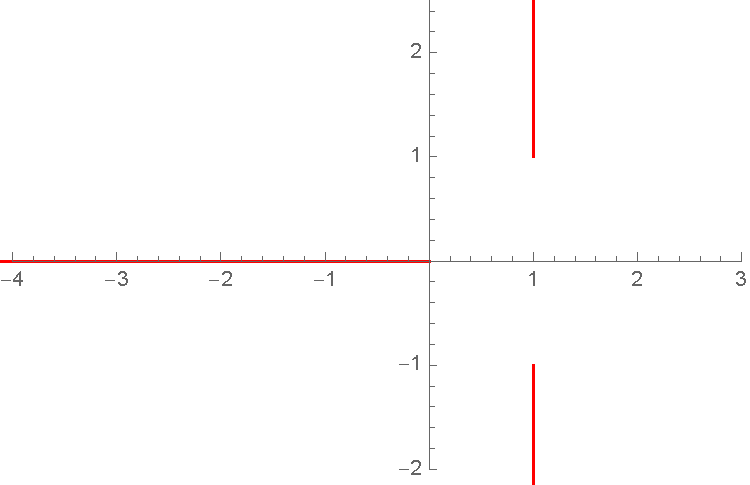
\includegraphics{Images/Sing.pdf}
%% \end{figure}
%% With this choice, as we will see in the next section, we are always able to find a path in the complex plane that stays away from singularities and does not cross any branch-cut.

%% \subsection{Paths in the phase-space}
%% \label{sec:paths}
%% In order to find a path in the complex plane that does not cross any singularity or branch-cut we can identified three different cases.

%% \begin{itemize}
%%     \item Starting and ending point on the real line. 
    
%%     In this case the choice for the path is quite simple and can be done in this way. Firstly we move up (or down depending on the Feynman prescription), then we move left or right depending on the relative position of the starting and ending points, and lastly we move down (or up). A path in the complex plane would look like this
%% \begin{figure}[!h]
%%     \centering
%%     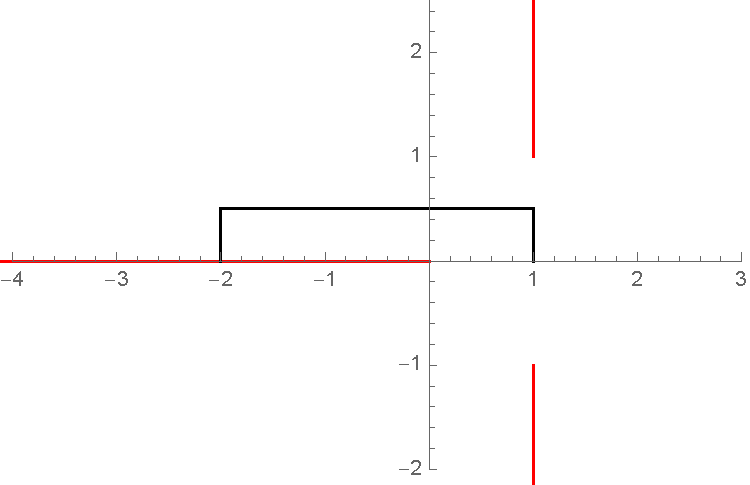
\includegraphics[scale=0.7]{Images/Sing2.pdf}
%% \end{figure}
%% As we said the choice of moving up or down depends on the Feynman prescription for the kinematic variable. In particular if the prescription is $+i\delta$ we move up, since we want to end up above the branch-cut, if it is $-i\delta$ we move down. One last thing to discuss is the height of the path, that is how much we move away from the real line. If there are no complex singularities than there is no risk of crossing any branch-cut when moving horizontally and the height can set arbitrarily to $1$. If there are complex conjugate singularities we can always find a \textit{safe strip}, in which we could move without crossing a cut. To this end we look at all the complex conjugates singularities and we consider the ones with the smallest imaginary part, that imaginary part will be the height of the safe strip. In the above example the safe strip is 
%% \begin{eq}
%% \text{Safe strip} = \{ z \in \mathbb{C}\; \text{s.t.}\; 0\le\text{Im}\; z \le 1\}.
%% \end{eq}
%% Inside this strip it is impossible to cross any cut and moving at half the height of the strip we can maximize the distance from singularities and hence increment the radius of convergence for each expansion.

%% \item Starting and ending point on the same side of the real line.

%% In this case we can simply reach vertically the line in the middle of the safe strip, move horizontally until we reach $\text{Re}\;s_{end}$ and then move vertically to $s_{end}$.
%% \begin{figure}[!h]
%%     \centering
%%     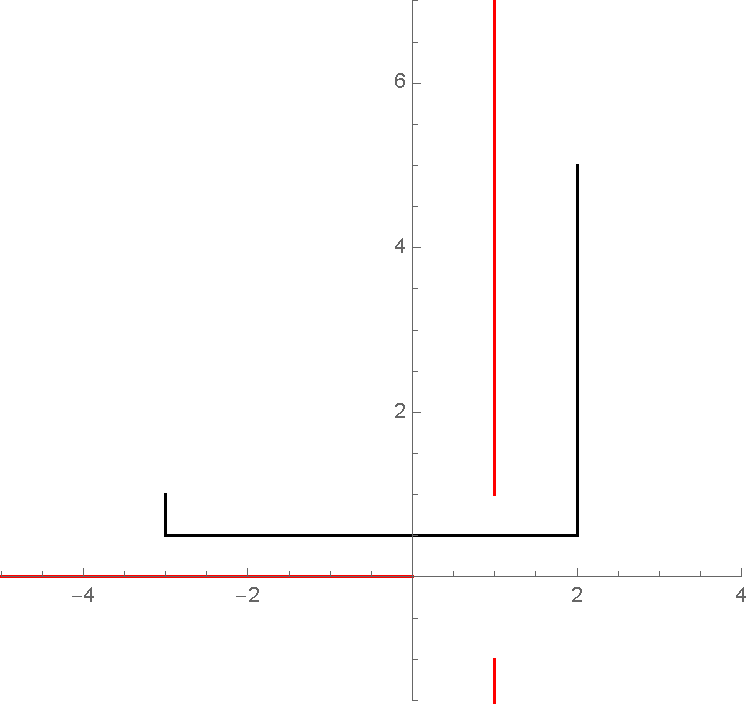
\includegraphics[scale=0.6]{Images/Sing4.pdf}
%% \end{figure}
%% Note that one of the points is complex and the other is real, the position of the real one is given by Feynman prescription, that is if $s_{start}=-3$, $s_{end}=3+3i$ and the Feynman prescription is $+i\delta$ we still fall into this case.

%% \item Starting and ending point on the opposite side of the real line.

%% In this case we need to cross the real line, and in doing this we must assure that we do not cross branch-cuts. We can identify a \textit{safe point} to cross the real line. If $s_{real,\;sing}$ is the set of real singularities, the safe point is $\max s_{real,\;sing} +1$. We can now move from $s_{start}$ to the safe-point and then from the safe point to $s_{end}$ using the ideas described in the first two cases.
%% \begin{figure}[!h]
%%     \centering
%%     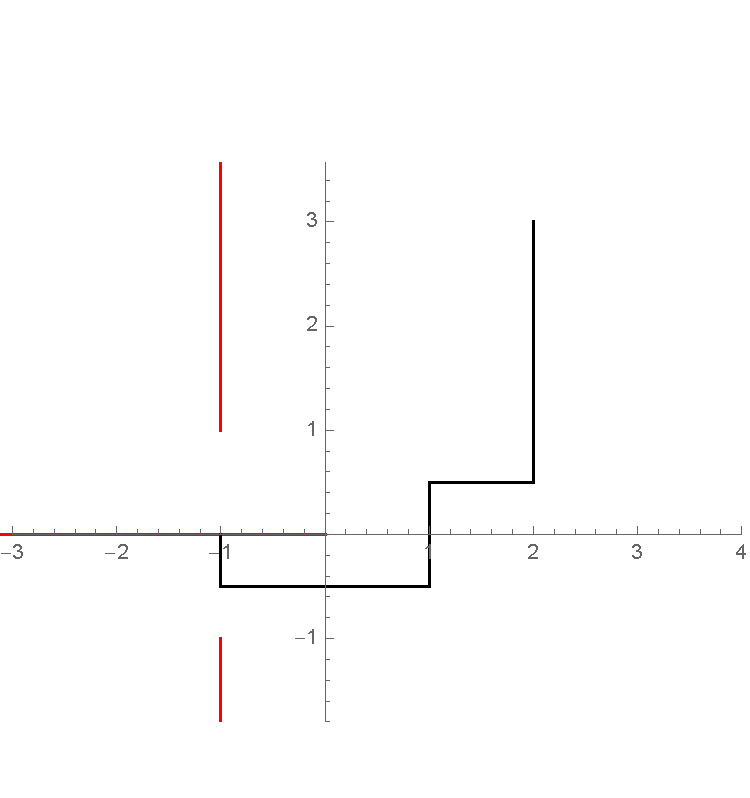
\includegraphics[scale=0.6]{Images/Sing3.pdf}
%% \end{figure}
%% \end{itemize}

